\documentclass[a4paper,english,twoside]{article}
\usepackage{a4,babel}
\usepackage[top=1in,bottom=1in,left=.75in,right=.75in]{geometry}
\usepackage[utf8]{inputenc}
\usepackage[T1]{fontenc}
\usepackage{graphicx,amssymb,amstext,amsmath,listings,color}
\usepackage{setspace,varioref,url,fancyhdr}
\usepackage{listings}
\usepackage{pxfonts}

\def\author		{Yasanka Sameera Horawalavithana(ens13sha)}
\def\subauthor			{Praneeth Nilanga Peiris(ens13pps)}
\def\course			{Distributed Systems, 5DV127, HT13}
\def\delivery		{Deliverable 02}
\def\trivialname	{GCom Middleware Project}
\def\tutor			{Francisco Hernandez-Rodriguez}
\def\title			{Report}
\def\myabstract	{}

\pagestyle{fancy}
\fancyfoot{}
\fancyhead[LO,LE]{\trivialname}
\fancyhead[RO,RE]{\today}

\fancyfoot[RO,LE] {\thepage}
\fancyfoot[LO] {\author}
\fancyfoot[RE] {\subauthor)}
\renewcommand{\footrulewidth}{0.4pt}

\lstset{language=Java,
    basicstyle=\ttfamily,
    keywordstyle=\bfseries,
    showstringspaces=false,
    morekeywords={syncronized}
}
%-----------------------------------------------------------
\begin{document}
%-----------------------------------------------------------
\begin{titlepage}

\newcommand{\HRule}{\rule{\linewidth}{0.5mm}}
\noindent
\HRule \\[0.4cm]
{ \huge \bfseries \trivialname - \title}\\[0.4cm] 
\HRule \\[1.5cm]

\noindent
\huge{\textbf{\course}} \\

\noindent
\huge{\textbf{\author}} \\
\huge{\textbf{\subauthor}} \\

\noindent
\huge{\textbf{\delivery}} \\

\noindent
\huge{\textbf{Tutors:}} \\
\huge{\textbf{\tutor }} \\ 
\huge{\textbf{Ewnetu Bayuh Lakew (lecturer)}} \\ 
\huge{\textbf{Cristian Klein (lecturer)r }} \\ 

\noindent
\huge{\textbf{\today}} \\
\\
\\
Running the program: 
\begin{verbatim}
1. $ cd ens13sha/edu/5DV147/GCom
2. Load modules: $ ant
3. Start a client: GUI Driven
4. Goto 3
\end{verbatim}






\end{titlepage}
%-----------------------------------------------------------
\thispagestyle{empty}
\pagenumbering{roman}


\tableofcontents
\thispagestyle{empty}

\newpage
\pagenumbering{arabic}
\renewcommand{\baselinestretch}{1.5}
\section{Introduction}
\paragraph{}
GCom middleware project demonstrates an implementation of middleware which is handling group membership issues, communication message exchange semantics, and message (re)ordering issues in group communication.
\subparagraph{}
GCom debug application simulates dropped, rearranged, or delayed packages, as this will allow us to test whether all modules are working correctly. GCom chat application is logically separated from debug application, so the debug view can be enabled upon request.
\paragraph{Tools Used}
Performance \& simplicity are important factors that has to be considered in choosing the appropriate technology for a particular application. Many developers of distributed systems prefer Java RMI as it's ease of use. Java RMI  auto-generates stubs and skeletons which hide the networking and data-marshalling aspects. Also it uses communications protocols that directly overlay the TCP/IP layer. Optionally Java RMI works with the HTTP protocol for requests and responses. As Java is easily ported we implemented GCom debug \& test applications using Java powered by RMI specifications.
 \subparagraph{}
 JUnit has been used for unit testing while Java Logging API is used to report runtime statistics \& Git as version control system.
 
\section{System Overview}
\paragraph{}
The GCom middleware consists of three (logical) modules, the group management mod-
ule, the communication module, and the message ordering module.
\subparagraph{}
The middleware handles communication between members of groups. Groups can be static or dynamic and they can have different message orderings to send messages using either basic or reliable multicast. Every member of the
group uses the same of these properties which are binded to their parent group. GCom middleware doesn't allow to have overlapping groups as they violate some algorithms used in implementation. Each group has a leader which has a reference in a registry. Clients can find groups and join them by getting a group list from the registry and contacting the leader.
\subparagraph{}
Communication in groups is done by passing messages. A message is usually
sent to the entire group, Messages are sent to only one
member in the group when (re)joining. Messages have a type so that application messages can be separated from system messages.

\begin{figure}[h]
\centering 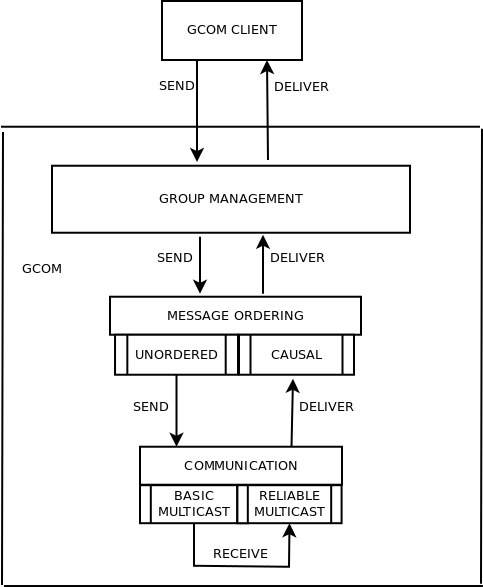
\includegraphics[width=300px]{High_Abstraction.png}
\caption{GCom Architecture.}
\label{fig:gcom_archi}
\end{figure}
\newpage
\section{Group management module}
\paragraph{}
Group management module handles the coordinations \& agreements related to group communication. In achieving distributed system properties(e.g. reliability, scalability, fault tolerance etc) group management module provides an upper layer to communicate between clients \& members of groups which are the destinations of messages sent with multicast operations from lower layers.
\subsection{Group memberships}
\paragraph{}
GCom middleware provides an interface to handle memberships of groups \& its members. We can create dummy logical groups prior to the assignment of members.We have implemented static groups as dynamic groups with some extra limitations.
The list of members in a static groups is created dynamically (by letting users join freely), the group is then freezed and the group becomes static. Only then can members can send messages to the group. This was the easiest way to implement static groups when we already had the dynamic ones. If only static groups would have been implemented they probably could have been created in a simpler way. But we initially implemented dynamic groups which it covers static groups as its subset. In dynamic groups, we allow members to (re)join or leave any time as the system does maintain the consistent state.
\paragraph{}
We avoid the common debugging utility of group creation where it has an automatically generated member assigned as leader. The first member who assigns to particular group will be selected as leader as there are no other members. The leader has an reference in the naming server, which is binded to its group name. Following members will get related reference from the naming server \& asks the group leader to join the group.(Figure: \ref{fig:add_mem})

\begin{figure}[h]
\centering 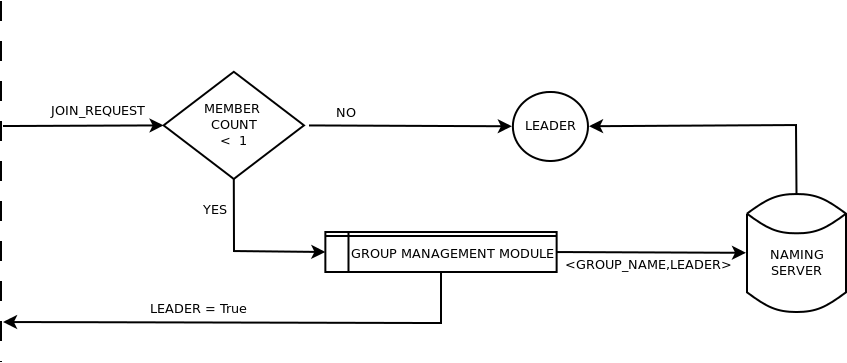
\includegraphics[width=300px]{Add_Member.png}
\caption{Add new member}
\label{fig:add_mem}
\end{figure}

\subsection{Group view}
\paragraph{}
The process maintain the view of its neighbor by updating the local member list from their joining order. This avoids the overhead of contacting the leader regularly when the process requires to call its neighbor. We find this is a necessary requirement as we need a consistent way to lookup neighbors without conflicting with \emph{deadlocks}. The process doesn't maintain any view of all groups. Also since we don't allow to have overlapping groups, the process can send messages to the members of its own group.

\subsection{Monitor}  
\paragraph{}
Group management module is responsible for detecting node failures as well as notifying changes of memberships to all group members. To simulate the failure of nodes we introduced \emph{Offline} feature where the particular node temporarily asks the leader to leave. The system gives \emph{Offline} nodes the chance to rejoin the group as maintaining its last consistent state. \emph{Offline} nodes are no longer there to receive group messages. When a node leaves the group, the leader multi-casts a message to the other members to update their group view.

\subsubsection{Election}
\begin{figure}[h]
\centering 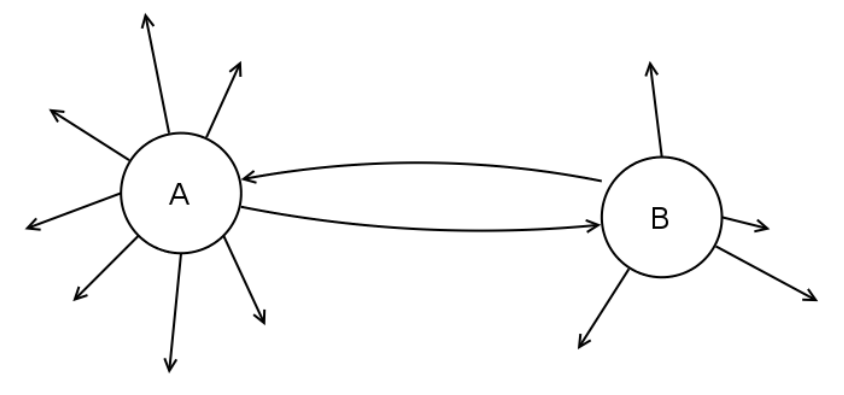
\includegraphics[width=300px]{Election.png}
\caption{Election}
\label{fig:election}
\end{figure}
\paragraph{}
Ring based election algorithm by Chang and Roberts is used to elect a single process acts as leader, which is the process with the largest identifier. To simplify our work we assign random identifier when new member creates, but we gave the possibility to change identifiers of members at system run time as to explore more test cases. As Figure: \ref{fig:election} shows, each process has a communication channel to its neighbor. The implementation doesn't modify the original algorithm as the assumptions will keep its chance to excuse pitfalls of the algorithm. 
\paragraph{}
In GCom debug application, there are implicit \& explicit ways to call for an election. If the group leader crashes the group will detect that no messages arrive to the leader and then elect a new leader. When a member (A in Figure \ref{fig:election}) detects that the leader is missing, an election of a new leader will take place. The member sets itself as leader of the group and sends
an election message for a collection of processes arranged in a logical ring. Ensuring algorithm semantics when a member is elected as new leader, it them binds its entry in the naming server. Leader then multicasts an elected message to all other members. 
\subparagraph{}
GCom guarantees that there will be no \emph{dead references} in the naming registry as the last member who may crash suddenly, unbind its reference from the naming server.

\subsubsection{Partitioning}
\paragraph{}
If a group is partitioned due to network segmentation, the destination node of any message will not be reachable. Since the communication module identifies this as a loss of any member, group management module partition the group \& update others about the modification. The partition with the leader will continue to work as before while other partition no longer receives messages from the leader. The other partition will elect a new leader when they discover that they don't receive any messages over time. It then registers new partitioned group with elected leader. So the new-comers now have two references in RMI registry where they can join.  

\section{Communication module}
\paragraph{}
This module is responsible for sending and receiving messages in between processes. This is based on multi-casting messages, where a sender sends a message to one or more other processes including itself. Since we are considering about the communication within a group, we only consider multi-casting among members in the same group.

\vspace{5mm}
\noindent
Note : Since this is a higher level communication, multi-casting is defined as performing P2P messages iterating through a recipients list.

\paragraph{}
There are three main types of communication modes based on multi-casting that we can implement in this project.

\begin{enumerate}
\item Basic unreliable multi-cast\\
This is the simplest way to send messages, where the sender just sends the messages to all other members and do not guarantee the delivery of them. If one or more recipients did not get the message, there is no other way it to receive it, unless the sender sends the message again because it will not get an acknowledgment.

\item Basic reliable multi-cast\\
In here, it guaranteed that a working process will eventually receive a message sent by another process. Simply explaining; when a process receives a message, it will multi-cast it to other processes before delivering it the upper layer.

\item Tree based reliable multi-cast\\
In here, all the messages are sent along a path in a tree structure such that a node only sends to its children or parent.
\end{enumerate}

\paragraph{}
Communication mode is defined when a group is created and all it's messages should be transfered according to that. We use \texttt{GroupDef} class to define it (by passing the corresponding mode to \textbf{commMode} parameter).

{ \begin{lstlisting}
GroupDef gd = new GroupDef(name, type, commMode, msgOrdering);
\end{lstlisting}}

Since every group has leader, it coordinates the critical messages and also communicates with the name server.

\paragraph{}
When a new member needs to join the group, it will first contact the \texttt{GroupManagement} module using \texttt{IGroupManagement} stub and get the reference to the group leader. If there is no leader (eg. empty group), it will be selected as the group leader explicitly. Then the group leader has to send notifications to other members saying that the group is modified. Then he multi-casts the message with updates of the group, so that members will update theirs.

\paragraph{}
A similar process is done when a member \textbf{wants to leave}, so it will send a message to the group leader and the group leader will update the group. Then it does a multi-cast a message containing updates to the group.
\paragraph{}
Or a member can invoke a multi-cast to start an election. For that, each member should have the view of the group; a list of references to other members with common order. And also if the group leader leaves the group, an election will be explicitly invoked by its neighbor.

\paragraph{}
The other scenario is when a member wants to send a message to one or more processes. Since it has the view of the group, it will multi-cast the message to the group.

\paragraph{}
In all these cases, subjective member will initiate the multi-cast and send P2P messages in separate threads. A \textbf{general} form of multi-casting can be represented as following.

{ \begin{lstlisting}
public syncronized void multicastMessage(IMember invoker,Message msg){
  LinkedList<IMember> membersList = invoker.getMembersList();
    for(IMember m : membersList){
      new Thread(){
        @override
        public void run(){
          m.send(msg);
        }
      }.start();
  }
}
\end{lstlisting}}

\section{Message Ordering module}
\paragraph{}
GCom uses two kind of message orderings: unordered \& causal. The message ordering modules have each been thoroughly tested with unit tests
to make sure that the algorithms works like intended. The algorithms and definitions of the ordering types can also be found in [1].

\subsection{Unordered}
\paragraph{}
This is the base class in message ordering module which doesn't require any order. The messages which are sent by one process may received by other processes at different order as they arrives. We use the service of working threads to implement multicast.

\subsection{Causal}
\begin{figure}[h]
\centering 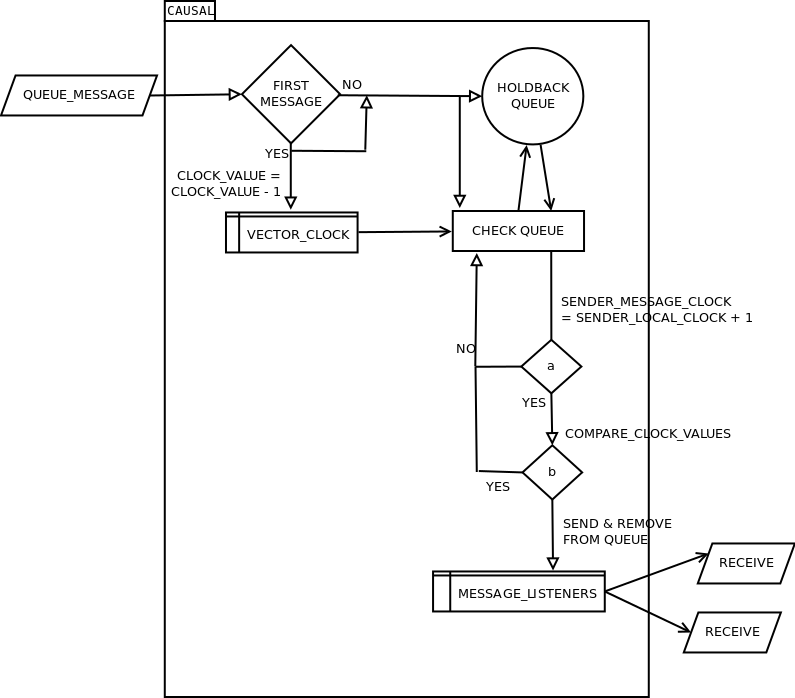
\includegraphics[width=10cm]{causal.png}
\caption{Causal message ordering algorithm}
\label{fig:causal}
\end{figure}
\paragraph{}
Assuming we have non-overlapping \& closed groups, the causal ordering algorithm proposed by Birman, is implemented here. The algorithm takes account of the \emph{happened-before} relationship only as it is established by multicast messages. Causal ordering will not be accounted for one-to-one messages.
\subparagraph{}
The algorithm works as shown in Figure: \ref{fig:causal}. When implementing above ordering technique, we uses hash vector clocks to keep the entries in the timestamps which counts the number of multicast messages from each process that happened-before the next message to be multicast. Each process maintains its own vector clock including timestamps values of all group processes. GCom is capable to obtain any type of multicast on given basic or reliable \& ordering.
\subparagraph{}
GCom debug application provides an informative GUI to show the messages delivered to specific ordering. Also the content of hold-back queues and other buffers are shown for clarity. For testing purposes, we present all messages waiting to be
sent or delivered as well as values of vector clocks and other counters. Also we provide a way to block or release messages from hold back queue explicitly.

\section{Testing}
First we created the basic structure for the middle-ware; Group Management, Members, Communication etc. Then we tested each block separately. The testing steps can be pointed out as following.

\begin{itemize}
\item Tested the RMI Server, where we keep the registries.
\item Member registration on the RMI server.
\item Manage groups with members, regardless of RMI server.
\item Bind the group to RMI server.
\item Election is tested separately. GUI.
\item Test message sending and message ordering.
\item Bind the system to the GUI.
\paragraph{}
\end{itemize}

We used many possible test-cases to test the modules and sub systems.
\paragraph{}
Then we combined related sub sections together and did a sub system testing. Then finally a full system test with different test cases for the system to check the robustness.

\paragraph{}
We used the native \texttt{Logger} class for logging errors.

\newpage
\section{GCom Application}
\paragraph{}
A debug application is created to demonstrate this Group Communication middle-ware. It will keep track of all the communication between processes.

\vspace*{5mm}
\noindent
There are two sides of this system.

\begin{enumerate}
\item RMI Server\\
All the groups and leaders are registered in the RMI registry running on this process. It may be running on a separate computer even on a separate network. All the information about groups and their leaders are stored here. The Group Management module is also running on this process. That module is also binded to the RMI registry as \texttt{IGroupManagement}, which is the stub to invoke methods of \texttt{GroupManagement} object.

\item Clients (Members)\\
Every client application is associated with a \texttt{Member} object, which represents the functionalities of a member in a group. This client has a Chat Window and a Debug Window. The chat window is used to send messages to other processes and debug window is used to track and manage those messages.
\end{enumerate}

\subsection{GCom Window}
\paragraph{}
This is the server side application to handle the RMI server and groups.

\paragraph{}
\begin{figure}[h]
\begin{center}
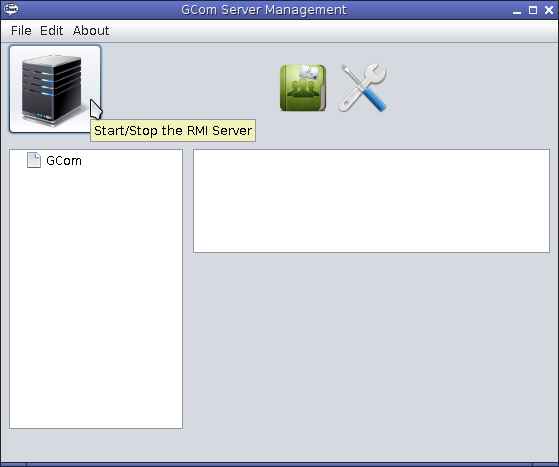
\includegraphics[width=400px]{GCom-1.png}
\caption{GCom Window}
\end{center}
\end{figure}

\paragraph{}
The RMI Server can be started by clicking on the \textit{Start/Stop RMI Server} button and it will prompt us to provide the $port$ to start it.

\begin{figure}[h]
\begin{center}
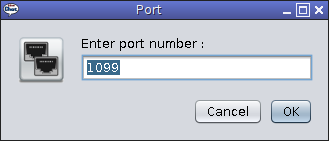
\includegraphics[width=250px]{GCom-Port.png}
\caption{GCom Window - Port}
\end{center}
\end{figure}

\paragraph{}
Then the RMI Server will be started and running. In background, it creates a \texttt{GroupManagement} object and bind it's stub to the \texttt{RMIServer}, which enables members to get information about groups when joining one of them.

\paragraph{}
This window lets us to creates new groups as well. We let Groups only to be created in the RMI Server.

\begin{figure}[h]
\begin{center}
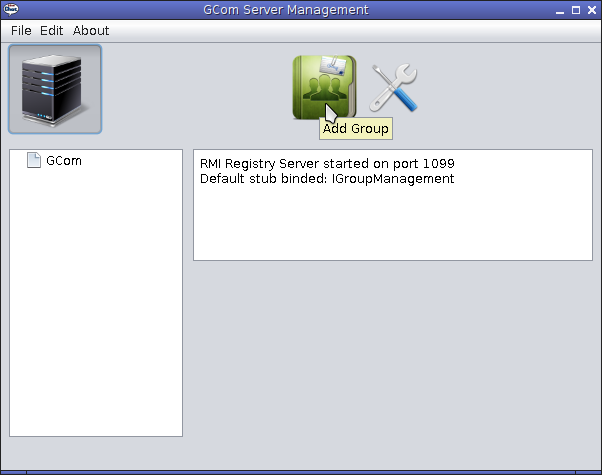
\includegraphics[width=400px]{GCom-NewGroup.png}
\caption{GCom Window - Create a Group}
\end{center}
\end{figure}
\newpage
\paragraph{}
Next we will be prompted to provide details about the \texttt{Group}.

\begin{figure}[h]
\begin{center}
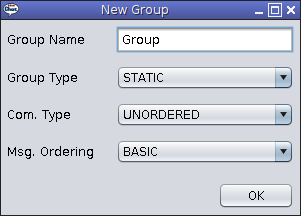
\includegraphics[width=250px]{GCome-Group.png}
\caption{GCom Window - Create a new Group}
\end{center}
\end{figure}

In here we have to proved \textit{Group Name}, \textit{Group Type}, \textit{Group Communication Mode} and \textit{Message Ordering Mode}. As mentioned in the Communication Module, this will create a \texttt{GroupDef} object and it will be send to the \texttt{GroupManagement} to create a \texttt{Group} object using it.

{ \begin{lstlisting}
GroupDef gd = new GroupDef(GroupName,GroupType,CommunicationMode,Message Ordering);
\end{lstlisting}}
\noindent
Then the GCom Window will be updated accordingly.

\begin{figure}[h]
\begin{center}
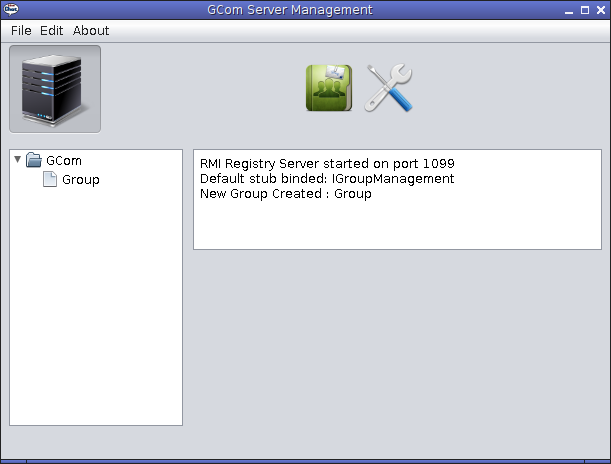
\includegraphics[width=300px]{GCom-2.png}
\caption{GCom Window - Group Created}
\end{center}
\end{figure}
\newpage

If a Group needs to be removed, we simply can right click on the Tree structure and select \textit{Remove Group} option. It will send \textit{kill} signals for all the processes belong to that group. It can be done by sending a kill message to the group leader and it will multi-cast that message to others. After multi-casting it, it will kill itself.
\begin{figure}[h]
\begin{center}
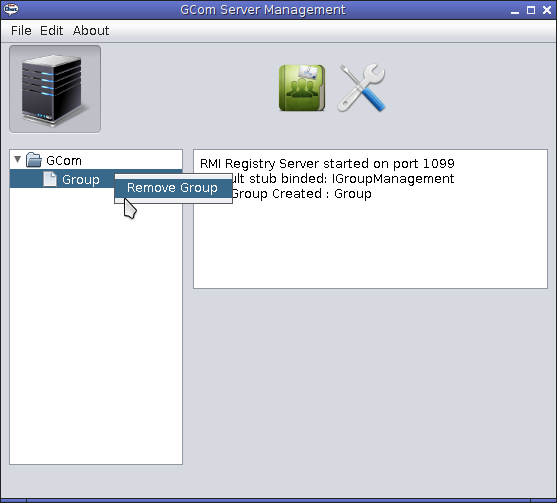
\includegraphics[width=350px]{GCom-RemoveGroup.png}
\caption{GCom Window - Remove Group}
\end{center}
\end{figure}

\subsection{Client Window}
\paragraph{}
When a member wants to join a Group, it will start the client application and it will prompt to \textit{Create Member} window. The host and the port of the targeting RMI Server should be provided in order to get group information and join the group.

\paragraph{}
When the Connect button is clicked, it will contact the RMI Server; \texttt{IGroupManagement} module more precisely and get the group information. Then you will see available groups in the below combo box. Then type a \textit{Member Name} and click \textit{Connect}.

\begin{figure}[h]
\begin{center}
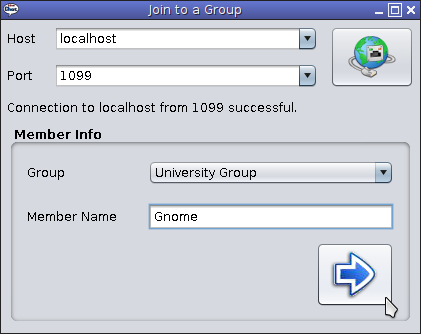
\includegraphics[width=300px]{Client-CreateMember.png}
\caption{Client Window - Create Member}
\end{center}
\end{figure}

\newpage
\subsubsection{Member Window}
\noindent
Then the \texttt{Member Window} will be prompted, where messages can be sent to other members (if there are). And we can get the \texttt{Debug Window} using \textit{Tools -> Debug}.
\noindent
If there are more members in the same group, there will be shown in the contacts list.

\begin{figure}[h]
\begin{center}
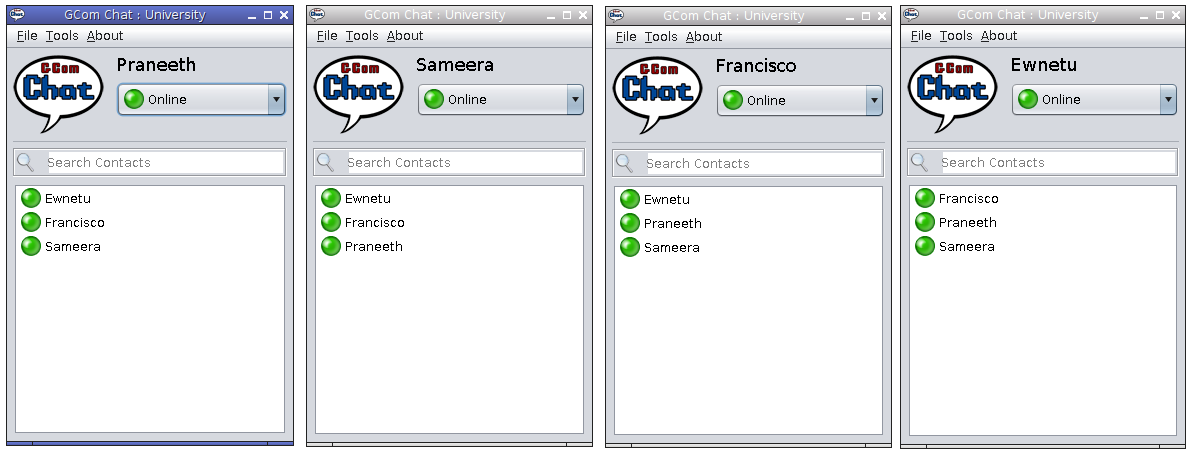
\includegraphics[width=490px]{Client-Chats.png}
\caption{Client - Member Window}
\end{center}
\end{figure}

\noindent
And the GCom Window will be updated accordingly.
\begin{figure}[h]
\begin{center}
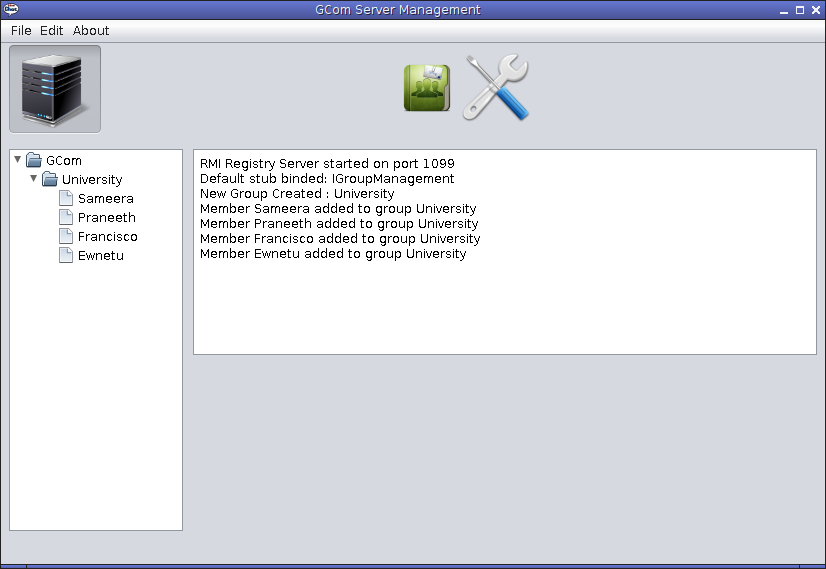
\includegraphics[width=350px]{GCom-MembersAdded.png}
\caption{GCom - Members Added}
\end{center}
\end{figure}

\paragraph{}
If a member want to leave, he can select the status as \textit{Offline} from the status list. Then he will not receive any further messages from the group. The reason is, he was removed from the group and no longer a part of the middle-ware. Whenever he wants to join again, he can select \textit{Online} as the status and he will be rejoined to the group and he will begin to receive messages from that moment on. But he will not get messages transmitted while he was offline.

\paragraph{}
This window provides a feature to search group members easily. Just type a name or even a part of a name in the search box.

\begin{figure}[h]
\begin{center}
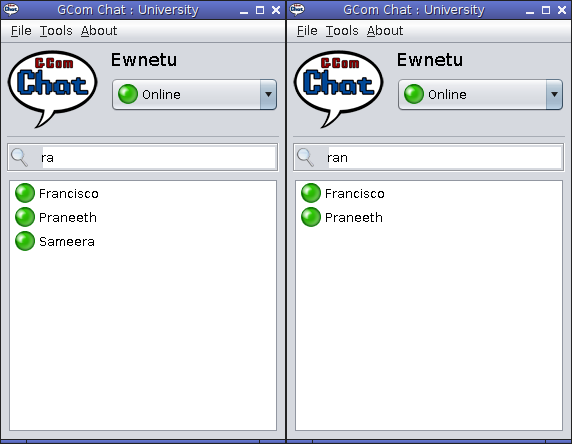
\includegraphics[width=250px]{Client-Search.png}
\caption{Client - Member Search}
\figurename{: Note that it shows containing "ra" and "ran" respectively.}
\end{center}
\end{figure}
\paragraph{}
If you want to send messages to a particular Member, just double click on a Contact on the Contact List. Then type a message and press Enter key.

\begin{figure}[h]
\begin{center}
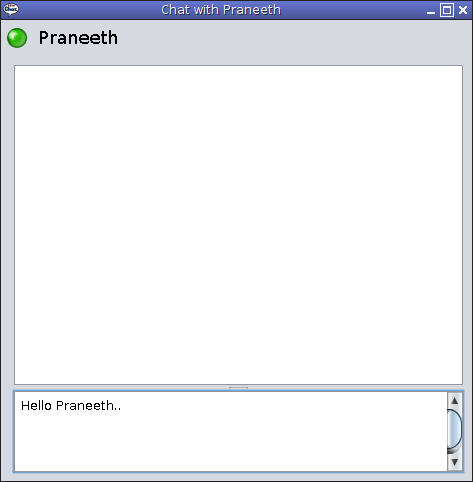
\includegraphics[width=150px]{Client-Chat-1.png}
\caption{Client - Chat with a Member}
\end{center}
\end{figure}
\paragraph{}
Then that message will be multi-casted and other processes will receive it. But it will be put into the hold back queue. So the sender will wait till acknowledgments receives. Whenever the acknowledgment from the target process receives, it will update the chat window as the message was sent. And when a process is releasing a message, it will update its chat window if the message was intended to him.

\begin{figure}[h]
\begin{center}
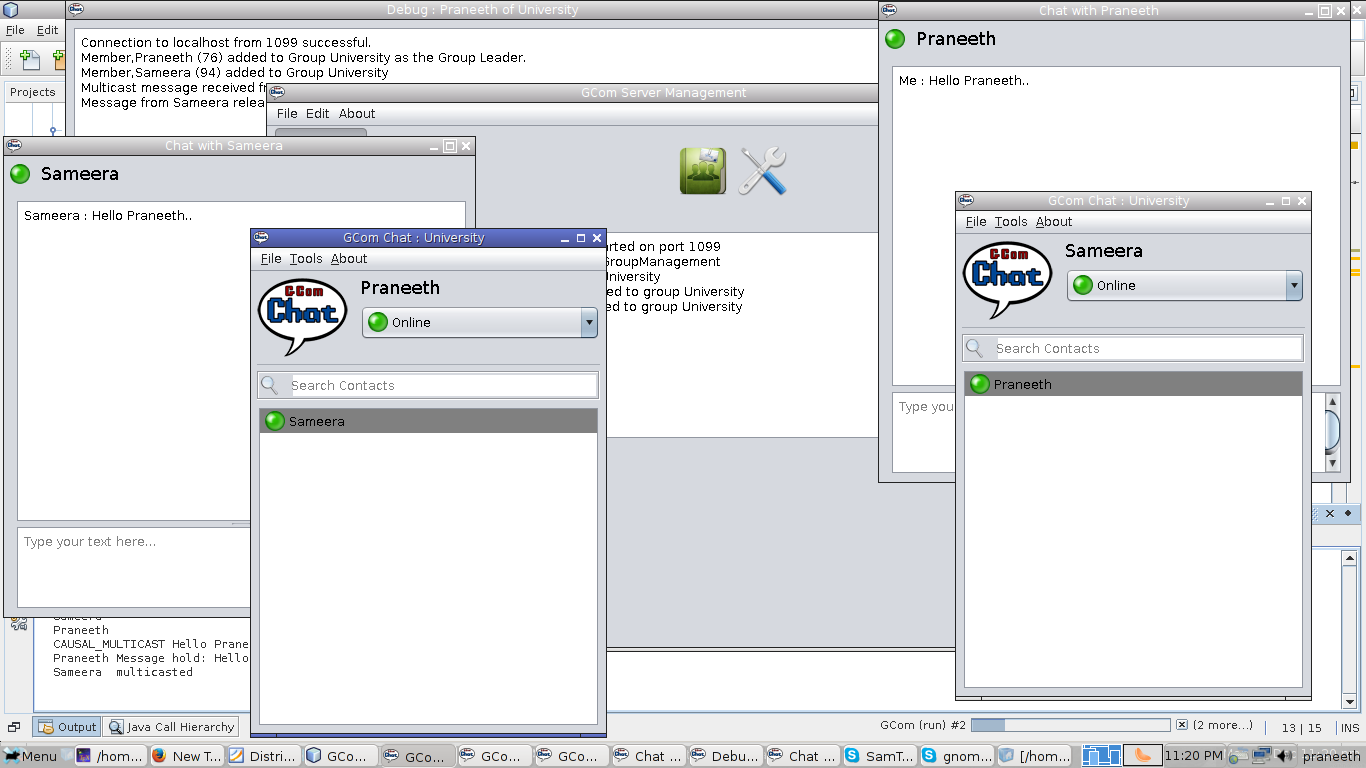
\includegraphics[width=430px]{Client-Chat.png}
\caption{Client - Final Chat Outputs}
\end{center}
\end{figure}

We can see the messages will be multi-casted through the middle-ware, but to implement this chat demonstration, we just check for the destination member.

\newpage
\subsubsection{Debug Window}
\paragraph{}
An important part of this project is debugging. This section is to illustrate how the messages are transmitted through the middle-ware.

\begin{figure}[h]
\begin{center}
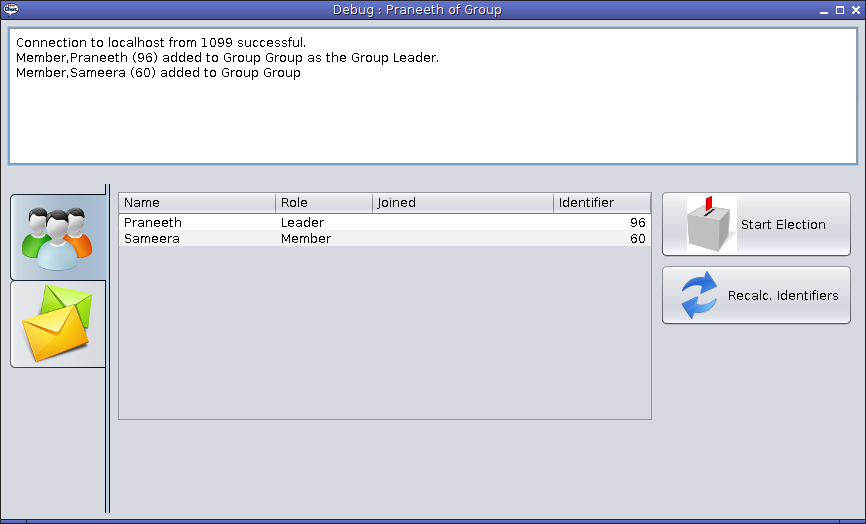
\includegraphics[width=350px]{DebugWindow-1.png}
\caption{Debug Window - Members}
\end{center}
\end{figure}

The table shows the current members, their role and their identifiers. An election can be called manually using \textit{Start Election} option. It will send a message to corresponding \texttt{Member} object to start a new \texttt{Election}.

\paragraph{}
An active process with the highest identifier (less system load) is selected as the group leader. Since we don't have a proper mechanism to calculate the system load for each process, we use some arbitrary values between 1 and 100 as the identifiers. So, if we need to start another election, it is better to re-calculate the process identifiers.

\paragraph{}
After an election, this table will be updated and will display the new leader and the status log will be updated with the passed messages.


\begin{figure}[h]
\begin{center}
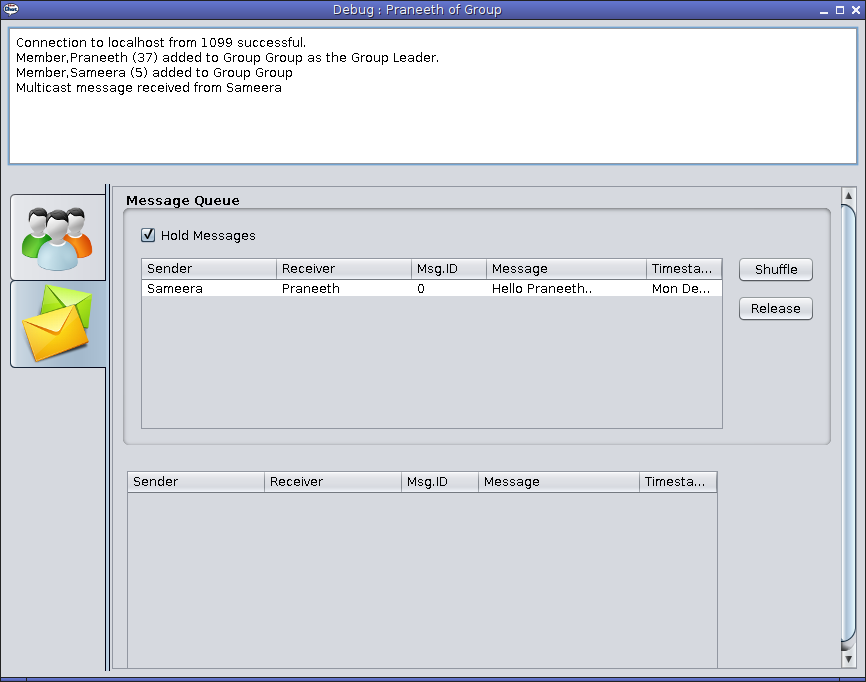
\includegraphics[width=450px]{DebugWindow-2.png}
\caption{Debug Window - Messages}
\end{center}
\end{figure}

\paragraph{}
This window show the messages being passed between processes. Since the communication is based on multi-casting, all the processes will get all the messages transmitted through the middle-ware. Right after a process receives a message, it will put that message into its \texttt{holding queue}. If the \textit{Hold Messages} is checked, they will not be released automatically and will need an explicit command to be released. If not, every message will be released right after received. All the released messaged will be added to the table in the below, which contains the delivered messages.

\paragraph{}
To demonstrate the message ordering in the middle-ware, we can shuffle the message, so that the order they got released will be changed.

\paragraph{}
In here, releasing a message simply means, sending an \textit{acknowledgment} to the sender and deliver it to the upper layer of the application. It may also multi-cast the message if the group uses reliable communication.
\newpage
\subsection{GUI Updating}
In this project, \textbf{GUIs are not updated with threads}. The most common and easiest way is to use a thread to listen to changes in the data objects. But it will cost a lot to maintain a smooth updates in the GUI.

\paragraph{}
But we have used Listeners provided by Java itself to detect changed in any kind of an object. The specialty of this concept is, it really doesn't need a an object to change in order to get a method invoked. We can virtually change an object to do it easily.

\paragraph{}
We have used \texttt{PropertyChangeSupport} class and create an object inside \texttt{Member} class. Then we create a method to add \texttt{PropertyChangeListener} to that \texttt{PropertyChangeSupport} object.

{\small { \begin{lstlisting}
public class Member extends UnicastRemoteObject implements IMember {
    // stuff here
    public void addPropertyChangeListener(PropertyChangeListener listener) {
        propertyChangeSupport.addPropertyChangeListener(listener);
    }
    // more stuff here
}
\end{lstlisting}}}

We have to add a \texttt{PropertyChangeListener} to this member class, so that it becomes sensitive to changes in properties.

{\small { \begin{lstlisting}
member.addPropertyChangeListener(new SignalListener(memWindow));
\end{lstlisting}}}

\noindent
In here, we have created a custom \texttt{PropertyChangeListener} class by implementing it.

{\small { \begin{lstlisting}
public class SignalListener implements PropertyChangeListener {
    private MemberWindow memWindow;
    public SignalListener(MemberWindow memWindow) {
        this.memWindow = memWindow;
    }
    public void propertyChange(PropertyChangeEvent evt) {
        if (evt.getPropertyName().equals("ElectionFinished")) {
            try {
                // Do whatever update you want to the GUI here.
                memWindow.electionCompleted((IMember) evt.getNewValue());
            } catch (RemoteException ex) {
                Logger.getLogger(SignalListener.class.getName()).log(Level.SEVERE, null, ex);
            }
        }
        // more stuff here..
    }
}
\end{lstlisting}}}

\noindent
Now executing this updates is very simple. Just fire this property change event inside the Member class.

{\small { \begin{lstlisting}
propertyChangeSupport.firePropertyChange("MemberLeft", parameters);
\end{lstlisting}}}

This is so much efficient comparing to using threads to do this work. And also these parameters inside custom \texttt{PropertyChangeListener} will not be transparent to the middle-ware, since it is implemented in the \texttt{Member} class, not in the \texttt{IMember} interface.

\section{Limitations}
\begin{itemize}
\item The RMI registry is a single point of failure. Since it crashes there will be no reference to the group \& no processes can find or join until it has restarted.
\item The system is not extended to handle overlapping groups, so therefore it's not allowed processes to join two groups at time
\item As we maintain states of temporarily left processes, we only allow them to rejoin to the same group
\item Assume that no processes will crash during an election
\item Assume that processes won't lie to cause malicious \& unexpected things
\item If large number of processes involve in multicast operation, this implementation is liable to suffer from \emph{ack-implosion}. Also multi-casting process's buffers will rapidly fill, and it's also liable to drop acknowledgments
\item Failures are detected as Remote Exceptions as we have not implemented heart-beat techniques 
\item The performance of GCom partially depends on the algorithms it used
\end{itemize}
\section{Future Work}

\paragraph{}

As we had limited time, we restricted our work to achieve minimum requirements within the deadline. But we're so much excited to extend this implementation further to cover whole gamut of message ordering techniques as well tree bases multi-cast. We would also like to develop another test application apart from chat service. Hopefully in the next phase of project deliverable, we may achieve some of our targets, also modified with GCom persistent technique.

\appendix
\section{Project plan} 
\label{app:projectplan}
\begin{tabular}{|l|l|p{7.5cm}|}
\hline
Date	&	Milestone	&	Content \\
\hline
05 Dec	&	Deliverable 1 due	&	Written project plan \\
12 Dec &	Milestone 1 &	Create all remote interfaces \\ 
						&&	Build data objects \\
						&&	Design GUI \\
14 Dec &	Milestone 2 & 	Implement basic group management module \\
15 Dec &	Milestone 2 & 	Implement basic communication module \\
17 Dec	&	Milestone 3 & 	Finalized group management module with election \\
20 Dec	&	Milestone 4 & 	Implement basic message ordering techniques. \\
21 Dec	&	Milestone 5 & 	Unit testing  \\ && Write the report.\\ && Make test protocol. \\
22 Dec	&	Finalization 	& Integration Test. Minor adjustments. \\
23 Dec	&	Deliverable 2 due 	& Final report \& implementation \\
24 onwards	&	Optimization 	& Extend project deliverables\\
06 Jan & Demonstration	& \\
\hline
\end{tabular}
\end{document}}
